\chapter{Navigation sensors} \label{chap:sensors}
This chapter gives an overview of the sensors used for localisation of an underwater vehicle and their characteristics. Underwater positioning can be based on usage of different types of sensors combined together in one system. The role of these sensors is to measure absolute position, velocities and heading/orientation. Localization is influenced with the development and performance of sensor devices. Sensors can be regarded as the means for managing the localization. Faster they are, more accurate they are, localization has more chances to perform better. Each sensor has its own reference system in which it operates. It is important to say that sensors output measurements with reference either in body frame (Figure ~\ref{fig:auv-axes}) - the one fixed to the object or in global frame (Figure ~\ref{fig:auv-positioning}). Basic navigation sensor set for a high-end AUV usually consists of depth sensor, magnetic compass, GPS device, LBL acoustic device, Doppler Velocity Log (DVL) and gyroscope, particularly fibre-optic gyroscope (FOG).   
\section{Inertial navigation system (INS)} \label{sec:ins}
Inertial navigation combines measurements of accelerometers and gyroscopes to track down the position and orientation of an object. Motion and rotation information obtained this way are processed in order to provide an estimate of objects location with respect to  initial reference. Recent INS configurations tend to consist of compact, more accurate and higher performance sensor devices.  
\subsection{Gyroscope}
Gyroscope is an INS sensor device that essentially measures orientation of the device. Although classic gyroscope measures orientation, modern gyroscopes are capable of measuring the angular rate. Gyroscopes can be mechanical, optical or MEMS gyroscopes. Underwater navigation uses fibre-optic gyroscope (FOG). FOG is based on measuring the interference of two light beams that pass through a coiled optical fibre in both directions. FOG provides quite precise information on rotation and its usage is intended for applications that demand higher performance. 
FOG can provide the angular information: rate of change of heading (yaw rate) and the yaw/heading itself. Both measurements can be used, depending on configuration. Since the sensor actually measures yaw rate (absolute measurement), yaw can be derived by integrating yaw rate in time. Disadvantage of such principally precise measurement, is that it is relative to previous yaw value and if that value turned out to be imprecise, drift can increase or contain a permanent bias. The KVH DSP-3000 device provides the Nessie vehicle with accurate angular rates.
\subsection{Doppler Velocity Log (DVL)}
DVL is intended to measure  velocities. Transceiver components mounted on the device, pointing downwards (towards the bottom) emit acoustic impulses which are expected to be reflected if the DVL is close enough to the bottom. In case of existing reflectance it is called having ``bottom-lock''. DVL usually has four transceivers. Each of them makes an angle with respect to the sea floor. If ``bottom-locked'', those four sensors undergo Doppler shift effect. Besides Doppler speeds, DVL measures roll, pitch and heading angles and fuses them together when computing surge, sway and heave velocity within the 3D speed vector in world referenced frame. The Teledyne Explorer PA DVL is used on Nessie AUV. This unit supplies the vehicle with altitude, surge, sway and heave velocities. Operation altitude ranges from 0.5 m to 80 m. Accuracy of the measured speeds is 0.7 cm/s when moving at the speed of 1 m/s.

\subsection{Magnetic compass} 
Magnetic compass provides 3D vector of local magnetic field. Magnetic compass points at magnetic north. Direction is determined so that it aligns with Earth's magnetic field. Important procedure before starting the compass usage is calibration. North direction as it appears on maps points to the geographic north (``true north''). That is the direction towards the rotation axis of the Earth. The direction of the \textit{magnetic north} does not overlap with the direction of the geographic north. Magnetic declination is an angle between magnetic north (measured by compass) direction and the true north direction (the one that maps refer to). Depending on location where the compass is used, magnetic declination can vary and the variation is different on different spots on the Earth's surface. Hence the calibration is necessary before usage. Magnetic compass gives measurements with slow variation in space. In addition, different magnetic effects caused by electric currents can affect the measurement, thus it is robust absolute measurement of heading, nonetheless, prone to noise. Nessie vehicle uses TCM 2.6 compass that precisely measures heading, pitch, and roll. Accuracy of the heading measurement is $0.8^{\circ}$.
\subsection{Depth sensor} 
Bathymetry system accomplishes depth measurement. It is possible to use the acoustic system for this purpose, however, bathymeter using pressure information tends to be more precise and trustable. Pressure sensor is standard piece of the equipment for an AUV. By measuring the pressure, it becomes possible to correlate the value of pressure with the value of depth. Device can frequently ascertain the absolute depth with good precision. A Keller Series 33X depth sensor measures the distance to surface having the depth range of 0 - 90 m and the accuracy of 0.05 m. 
\subsection{Global Positioning System (GPS)}
This well known satellite-based navigation system provides position information anywhere on the Earth surface or in the air, reasonably close to the surface. Due to absorption of electromagnetic waves in the water GPS signal is not available underwater. Despite the fact that GPS is not available, vehicles are equipped with GPS receiver intended to be used for initial position information before submerging or for occasional position updates if the vehicle temporarily goes back to the surface. Precision of the GPS position information can vary. Namely, range of the standard deviation errors can have the order of 25.27 m \cite{farrell98}. Such huge deviation can cause significant inaccuracies in navigation. An example of the influence of GPS imprecision was shown in Figure ~\ref{fig:with-gps}. Differential GPS (DGPS) \cite{farrell98} can be used in situations when better precision is needed.
\section{Acoustic positioning system}
Provides the absolute position, a ground-based reference. Principal way of exchanging the information through the environment is sound wave. Long baseline (LBL) is used for measuring position with respect to several tethered beacons with known position, placed in water (Section \S~\ref{sec:acoustic}). It can be understood as the extension of the GPS information below the water surface. Such system employs acoustic signals to measure the distances. Vehicle uses the acoustic transponder to send the acoustic wave (``pinging''). The wave reaches beacon and reflects back to the vehicle . LBL system consists of transceiver and array-arranged collection of beacons. LBL transceiver pings each of the beacons and detects the signal travel time in order to calculate the distance, knowing the speed of sound in water. Distances from the beacons are combined together in triangulation method. Triangulation makes it possible to determine the position of the robot in the network of fixed beacons. LBL position update can introduce the outliers that need to be rejected or filtered. 
%As stated in some practical implementations (\cite{blain03}), DVL and acoustic sensor perform ...
\begin{figure}
  \centering
    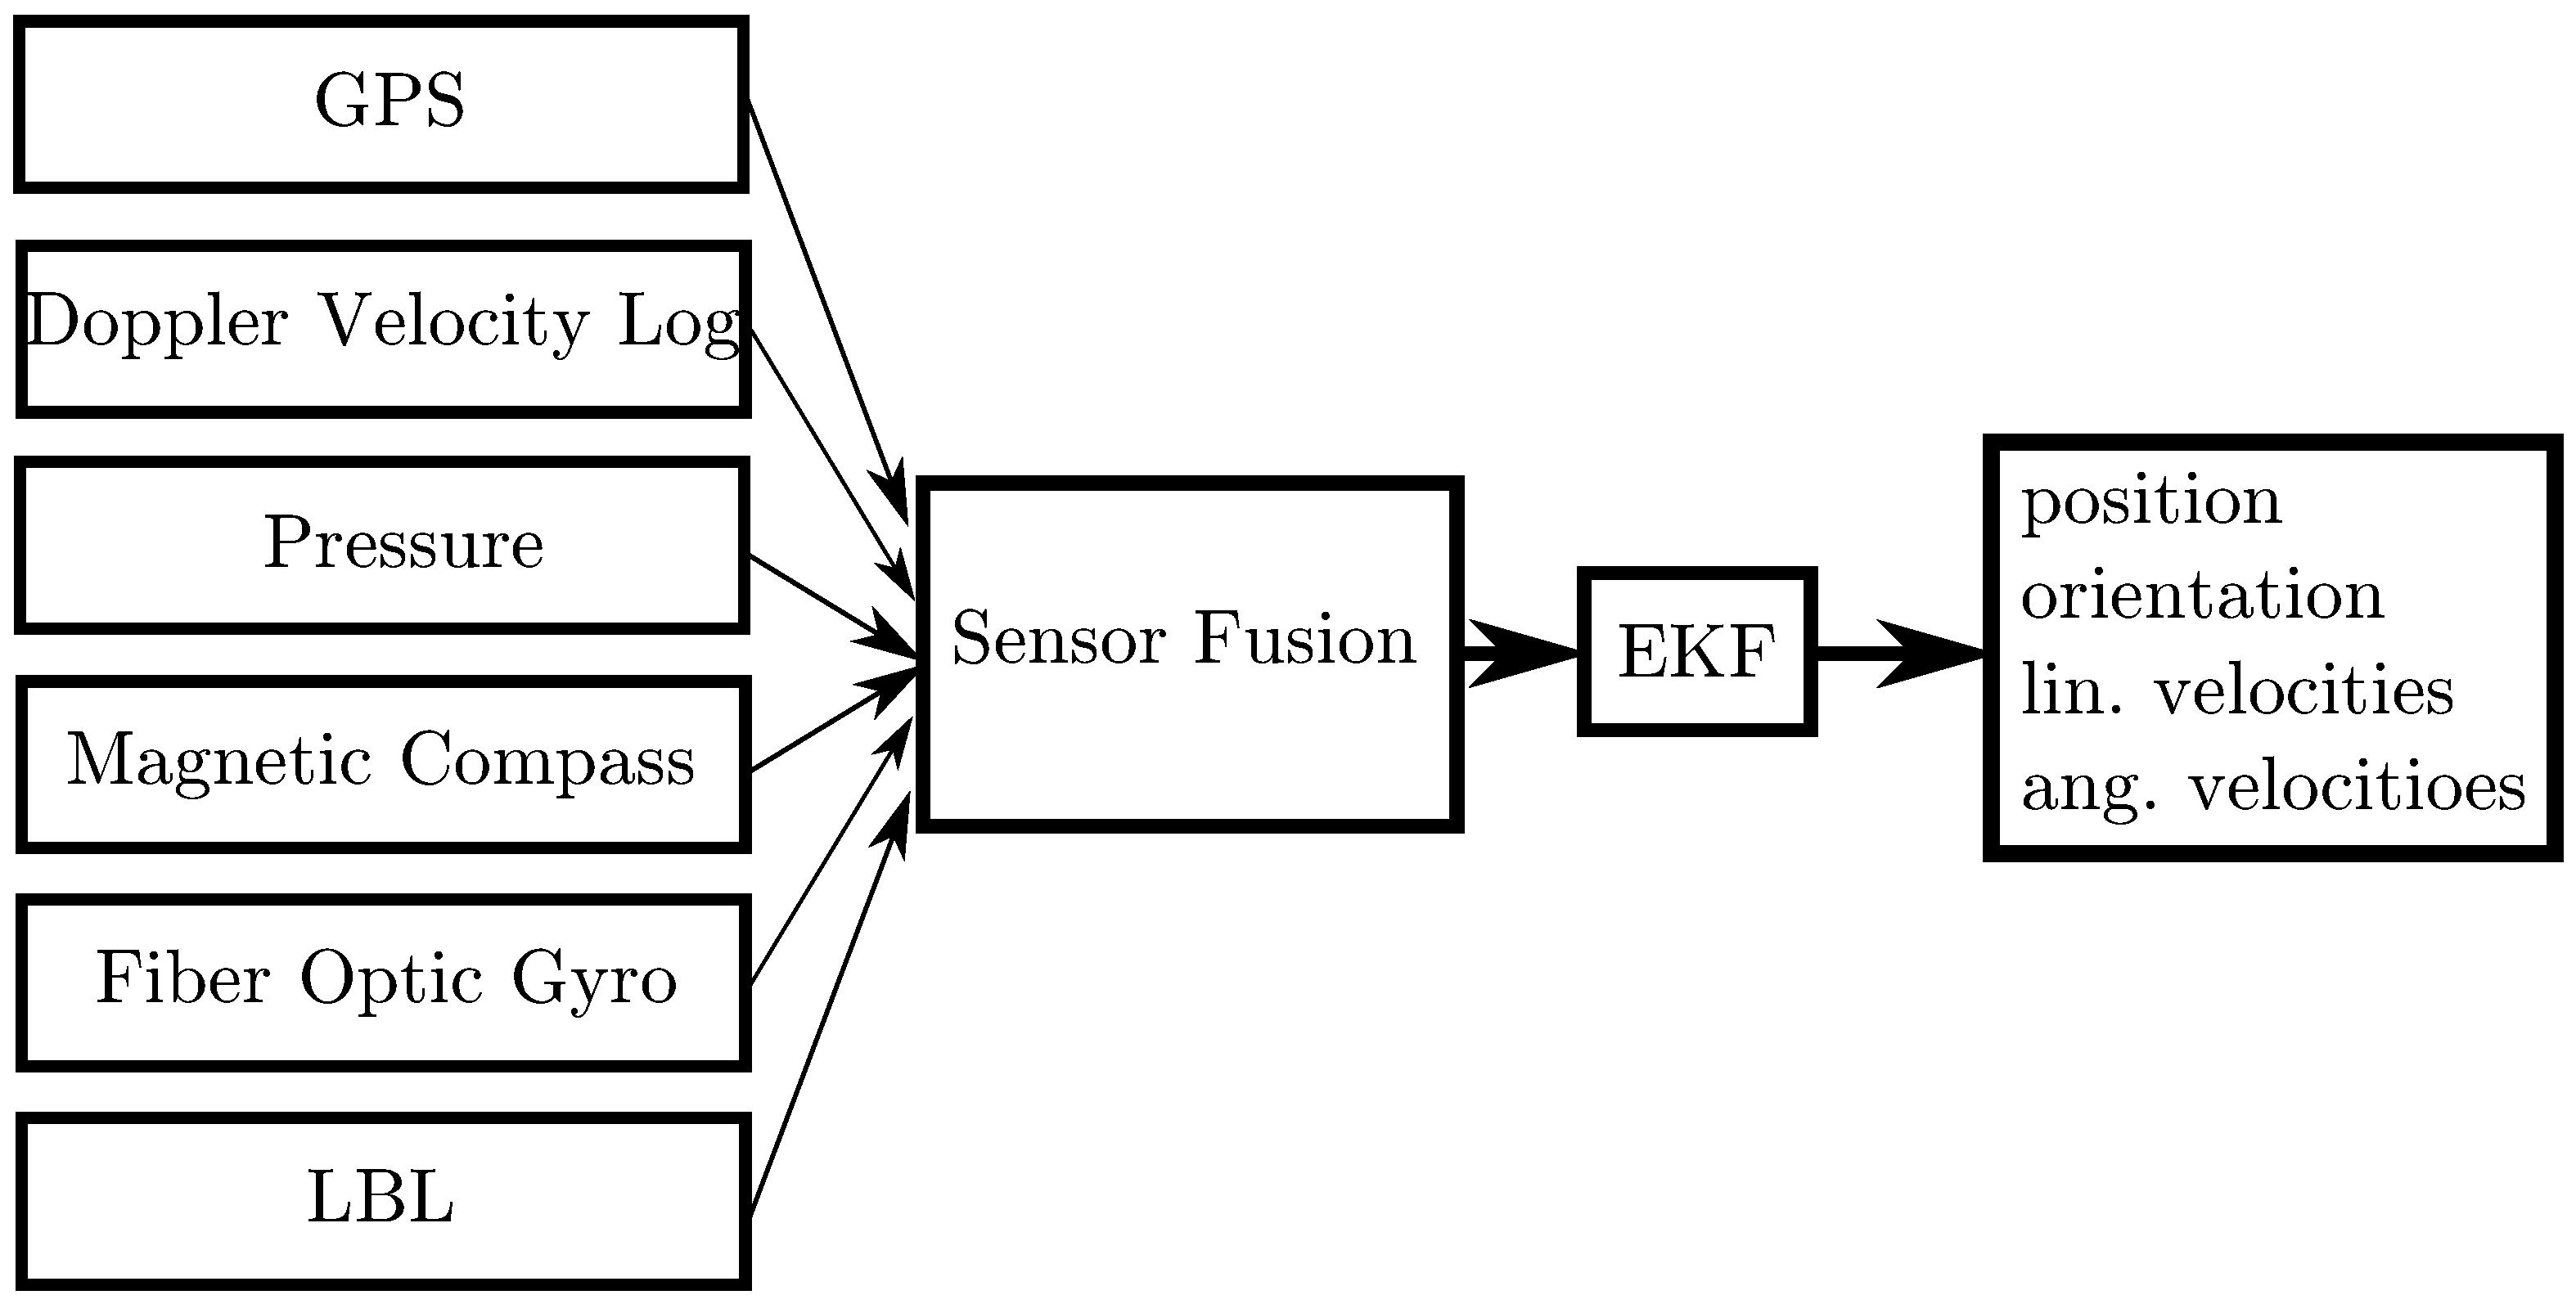
\includegraphics[width=0.65\textwidth]{methodology/fig/fusion.eps}
  \caption{Sensor fusion diagram.}
\vspace{-10pt}
\label{fig:sensor-fusion}
\end{figure}
\begin{table*}
\centering
	\caption{Navigation sensors characteristics.}
	\label{tab:sensors-char}
\begin{tabular}{llllll}
\toprule
Sensor      &     Measures     &   Update rate   &   Precision	  &    Accuracy    &    Range  \\
\midrule
\multirow{4}{*}{Pressure} & \multirow{2}{*}{depth} & \multirow{2}{*}{10 Hz} & 0.0002 $bar$ & 0.005 $bar$ & $0 - 10$ $bar$  \\
         	              &   &                         & (0.002 $m$)  &  (0.05 m)   & (0-90 $m$ in water) \\ 
                          & \multicolumn{5}{c}{\contra heave velocity is calculated by deriving depth in time - higher possibility of error} \\ 
        	              & \multicolumn{5}{c}{\pro distance from surface available no matter of distance from the seabed} \\                      
\midrule
\multirow{6}{*}{Compass}&yaw(heading)&\multirow{3}{*}{10 Hz}& $0.1^{\circ}$ & $0.8^{\circ}$ &              \\
         	            &pitch       &                       &               &               & tilt $\pm 50 ^{\circ}$  \\
         	            &roll        &                       &                &                &                    \\
  & \multicolumn{5}{c}{\pro absolute measure of heading - no drift } \\
  & \multicolumn{5}{c}{\contra needs magnetic north correction (due to magnetic declination)} \\
  & \multicolumn{5}{c}{\contra prone to magnetic disturbance} \\
\midrule
\multirow{2}{*}{FOG} & \multirow{2}{*}{yaw rate} & \multirow{2}{*}{5Hz} & \multirow{2}{*}{$ < 1^{\circ} / hr$} & \multirow{2}{*}{$\pm 20^{\circ} / hr$} & \multirow{2}{*}{$\pm 375 ^{\circ}/s$} \\
     &          &           &           &         &         \\
 & \multicolumn{5}{c}{\pro high accuracy in heading measurement, compared to compass} \\
 & \multicolumn{5}{c}{\contra drifts over time, needs correction for the Earth rotation} \\
\midrule
\multirow{3}{*}{DVL} & surge velocity & \multirow{3}{*}{10 Hz} & \multirow{3}{*}{$0.1\frac{cm}{s}$} & $ \pm 0.7\frac{cm}{s}$ at $1\frac{m}{s^{4}}$ & \multirow{3}{*}{$\pm 9.5\frac{m}{s}$} \\
         	        &sway velocity&                        &                                    & $ \pm 1.9\frac{cm}{s}$ at $3\frac{m}{s^{4}}$ &                                  \\
         	        &heave velocity &                      &                                    & $ \pm 3.0\frac{cm}{s}$ at $5\frac{m}{s^{4}}$ &                              \\
 & \multicolumn{5}{c}{\contra relative measurement of velocity} \\
 & \multicolumn{5}{c}{\contra requires depth - looses lock at $0.6$ $m$ altitude resulting in no output} \\
\bottomrule
\end{tabular} 
\end{table*}